\chapter{Lecture 4}

This lecture is about \texttt{Linear Classifiers and Basis Expansion
[LDA, QDA, Logistic regression, Splines]} where chapter \texttt{ESL Chapter 4.3, 4.4, 5.1
and 5.2} should be looked upon.

\cite{lecture4}

\section{Chapter 4.3}

Here we will talk about the LDA

\section{Chapter 4.4}

This chapter will be about Logistic Regression

\section{Chapter 5.2}

And finally this chapter will be about the piecewise polynomials and splines.

\section{Linear Discirminant Analysis}

$f_k(x)$ is the class-conditional density of X in class $G = k$ and let $\pi_k$ be the prior probability of class $k$ with $\sum_{k=1}^{K}  \pi_k = 1$. Then we have the probability of class $k$, given observation $x$ as

\[
    P(G = k | X = x) = \frac{f_k (x) \pi_k}{\sum_{\ell = 1}^{K} f_\ell (x) \pi_\ell}
\]

where $f_\ell$ is distribution for class $\ell$ and $\pi_\ell$ is a priori probability for class $\ell$

We need a stochastic model for data to calculate probabilities, and we assume that the data come from a different Gaussian distributions.

A straight line will be our decision boundary.

We look at the log-odds-ratio for the two classes $k$ and $\ell$

\[
    \log \frac{P(G = k | X = x)}{P(G = \ell | X = x)} = \log \frac{f_k(x)}{f_\ell (x)} + \log \frac{\pi_k}{\pi_\ell}
\]

where $f(x) = \frac{1}{(2 \pi)^{p/2} |\Sigma_k|^{1/2}} \exp(-\frac{1}{2} (x - \mu_k)^T \Sigma^{-1}_k (x - \mu_k))$ which is the multivariate Gaussian with a common covariance matrix $\Sigma_k = \Sigma \forall k$

This linear log-odds function implies that the decision boundary between classes $k$ and $\ell$ is linear in $x$ in $p$ dimensions a hyperplane $a + x^T b = 0$

The decision boundary becomes

\[
    \log \frac{\pi_k}{\pi_\ell} - \frac{1}{2} (\mu_k + \mu_l)^T \Sigma^{-1} (\mu_k - \mu_l) + x^T \Sigma^{-1}(\mu_k - \mu_l)
\]

From this equation we see that the linear discriminant functions

\[
    \delta_k(x) = x^T + \Sigma^{-1} \mu_k - \frac{1}{2} \mu_k \Sigma^{-1} \mu_k + \log \pi_k
\]

are an equivalent description of the decision rule with $G(x) = \arg \max\limits_k \delta_k (x)$

We do not know the parameters of the Gaussian distributions, and will need to estimate them using our training data.

\[
    \hat{\pi_k} = N_k / N
\]

where $N_k$ is the number of class-$k$ observations

\[
    \hat{\mu_k} = \sum_{g_i = k} x_i / N_k
\]

and

\[
    \hat{\Sigma} = \sum_{k=1}^{K}\sum_{g_i = k} (x_i - \hat{\mu_k})(x_i - \hat{\mu_k})^T / (N - K)
\]

As seen in \cite[p.~110]{friedman2016elements}

If we have more than two classes, then one decision line for each of classes and one discriminant function for each class.

So Linear discriminant analysis assumes that the covariance structures are equal.

When we drop this restriction we get quadratic discriminant
analysis, QDA, and the decision boundaries becomes non-linear.

\begin{figure}[H]
  \centering
  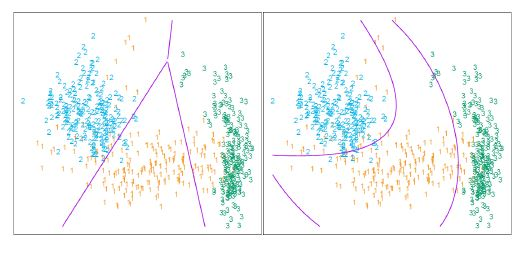
\includegraphics[width=0.9\textwidth]{QDAvsLDA}
\end{figure}

\section{Regularized discriminant analysis}

It takes a lot of observations to estimate a large covariance matrix
with precision. Three increasingly harsh regularizations are available

From lecture \cite[p.~15]{lecture4} We make a compromise between LDA and QDA which allows to shrink the seperate covariance of QDA toward a common covariance as in LDA.

\[
    \hat{\Sigma}_k (\alpha) = \alpha \hat{\Sigma}_k + (1 - \alpha) \hat{\Sigma}
\]

where $\hat{\sigma}$ is the pooled covariance matrix as used in LDA and $\alpha \in [0, 1]$

Then shrink the covariance toward its diagonal

\[
    \hat{\Sigma}_k ( \gamma) = \gamma \hat{\Sigma} + (1 - \gamma) \text{diag}(\hat{\Sigma})
\]

Similar modifications allows $\hat{\sigma}$ itself to be shrunk toward the scalar covariance structure

\[
    \hat{\Sigma}_k ( \gamma) = \gamma \hat{\Sigma} + (1 - \gamma)\hat{\Sigma}^2 \bm{I}
\]

In these situations the features are high-dimensional and correlated, and the LDA coefficients can be regularized to be smooth or sparse in the original domain of the signal.

\section{Reduced rank discriminant analysis}

So far we have discussed LDA as a restricted Gaussian classifier. Part of its popularity is due to an additional restriction that allows us to view informative low-dimensional projections of the data.

Hence, this technique is very useful for illustrating class separation.

If K = 3, for instance, this could allow us to view the data in a two-dimensional plot, color-coding the classes. In doing so we would not have relinquished any of the information needed for LDA classification. More on \cite[p.~114]{friedman2016elements}

\section{Logistic Regression}

The logistic regression model arises from the desire to model the posterior probabilities of the K classes via linear functions in x, while at the same time ensuring that they sum to one and remain in [0, 1].

From lecture \cite[p.~21]{lecture4} we want to derive expressions for the two class problem, i.e. $P(G = red | X = x)$ and  $P(G = blue | X = x)$ when $\log \frac{P_r}{P_b} = \beta_0 + x \beta$

Logistic regression models are usually fit by maximum likelihood, using the conditional likelihood of $G$ given $X$. So the likelihood for $N$ observations is

\[
    L ( \beta_0, \beta) = \prod_{i=1}^{N} P(G = g_{x_i} | X = x_i)
\]

as seen in lecture \cite[p.~22]{lecture4}. Where the log-likelihood is

\[
    \ell ( \theta ) = \sum_{i=1}^{N} \log  P(G = k | X = x_i; \theta)
\]

We wish to maximize the log-likelihood, wrt to $\beta$ where $\beta = \{\beta_0, \beta\} $


\[
    \ell (\beta_0, \beta) = \sum_{i=1}^{N} (\beta_0 + x_i \beta) - \log ( 1 + \exp(\beta_0 + x_i \beta))
\]

This is known as maximum likelihood and the result is called logistic regression.

To maximize the log-likelihood, we set its derivatives to zero

\[
    \frac{\partial \ell (\beta)}{\partial \beta}  = 0
\]

and to solve this equation we use the Newton-Raphson algorithm, which requires the second derivative or Hessian Matrix \cite[p.~121]{friedman2016elements}

From lecture \cite[p.~29]{lecture4} then the reason to use logistic regression is

\begin{itemize}
  \item Statistics
  \begin{itemize}
    \item Identify variables important for separating the classes
    \begin{itemize}
      \item Biostatistics and epidemiology
    \end{itemize}
  \end{itemize}
  \item Classification
  \begin{itemize}
    \item Predict class belonging of new observations
    \begin{itemize}
      \item For example spam/email or diseased/healthy
    \end{itemize}
  \end{itemize}
  \item Risk prediction
  \begin{itemize}
    \item Estimate probability (risk) for each class
    \begin{itemize}
      \item Fraud detection in insurance claims
    \end{itemize}
  \end{itemize}
\end{itemize}

\subsection{Interpreting the coefficients}

The example is we have a model of lung cancer (yes/no) as a function of smoking (number of cigarettes per day).

If $\beta = 0.02$, then a unit increase in smoking (one extra cigarette) means an increase in lung cancer risk of $\exp(0.02) \approx 1.02 = 2\%$ from lecture \cite[p.~30]{lecture4}

More can be seen on \cite[p.~124]{friedman2016elements}

\section{L1 Regularized Logistic Regression}

If we have few observations, low $n$, and high dimension, high $p$ data is a problem also for logistic regression.

One solution is an elastic net regularization of the likelihood.

\[
    \max\limits_{\beta_0, \beta} \left\{\sum_{i=1}^{N} \left[ y_i (\beta_0 + \beta^T x_i) - \log (1 + \exp(\beta_0 + \beta^T x_i)) \right] - \lambda \sum_{j=1}^{P} |\beta_j | \right\}
\]

As with the lasso, we typically do not penalize the intercept term, and standardize the predictors for the penalty to be meaningful.

The equation is concave and a solution can be found using nonlinear programming methods.

\begin{itemize}
  \item Logistic regression is more robust than LDA
  \begin{itemize}
    \item It relies on fewer assumption
    \item When is this a bad thing when compared to LDA?
  \end{itemize}
  \item Logistic regression handles categorical variables better than LDA
  \item Observations far away from the boundary are down-weighted
  \begin{itemize}
    \item You will have a look at how this works during the exercises
  \end{itemize}
  \item Breaks down when classes are perfectly separable
  \item Easy to interpret and explain
  \item Surprisingly often hard to beat
  \item Can be combined with regularization of parameters (n < p)
  \item Can be generalized to multi-class problems
\end{itemize}

\section{Basic Expansions and Regularization}

\begin{itemize}
  \item We are not limited to use our data as they are
  \item Linear models
  \begin{itemize}
    \item Easy to interpret
    \item First order Taylor expansion of non-linearities
    \item Might be ok even for non-linear data if we have a few observations
  \end{itemize}
  \item Non-linear problem - transform data and use linear model
  \begin{itemize}
    \item $h_m  (X) = X^2_j$ and $h_m (X) = X_j X_k$
    \item $h_m (X) = \log (X_j )$ or $h_m (X) = \sqrt{X_j}$
    \item $h_m (X) = \frac{X - m_X}{s_X}$ (always used when using regularization
    \item $h_m(X_{(i)} = i$ sort data $X_{(1)} \leq X_{(2) } \leq ...$ and use the rank
    \item Either replacing $X$ with $h_m(X)$ or expanding $\{X, h_m(X)\}$
  \end{itemize}
\end{itemize}

In this chapter and the next we discuss popular methods for moving
beyond linearity. The core idea in this chapter is to augment/replace the vector of inputs $X$ with additional variables, which are transformations of $X$, and then use linear models in this new space of derived input features.

We denote by $h_m (X)  : \mathbb{R}^p \rightarrow \mathbb{R}$ the mth transformation of $X, m = 1, ..., M$, we then have the model

\[
    f(X) = y = X \beta = \sum_{m = 1}^{p} \beta_i x_i \rightarrow \sum_{m = 1}^{M} \beta_i ' h_i (X)
\]

Sometimes the problem at hand will call for particular basis functions $h_mm$, such as logarithms or power functions.More often, however, we use the basis expansions as a device to achieve more flexible representations for $f(X)$.

From the lecture \cite[p.~47]{lecture4} then we wish to have cubic splines.

Then we wish to have $h_0 (x) = 1$, $h_1 (x) = x$, $h_2 (x) = x^2$, $h_3 (x) = x^3$, $h_4(x) = (x-5)^3_+$ and so on.

We often prefer smoother functions, and these can be achieved by increasing the order of the local polynomial. Cubic splines have continuous first and second derivatives at the knots, which means smooth functions. We should be able to obtain non-linear functions with a linear model. 